\documentclass{article}\usepackage[]{graphicx}\usepackage[]{color}
%% maxwidth is the original width if it is less than linewidth
%% otherwise use linewidth (to make sure the graphics do not exceed the margin)
\makeatletter
\def\maxwidth{ %
  \ifdim\Gin@nat@width>\linewidth
    \linewidth
  \else
    \Gin@nat@width
  \fi
}
\makeatother

\definecolor{fgcolor}{rgb}{0.345, 0.345, 0.345}
\newcommand{\hlnum}[1]{\textcolor[rgb]{0.686,0.059,0.569}{#1}}%
\newcommand{\hlstr}[1]{\textcolor[rgb]{0.192,0.494,0.8}{#1}}%
\newcommand{\hlcom}[1]{\textcolor[rgb]{0.678,0.584,0.686}{\textit{#1}}}%
\newcommand{\hlopt}[1]{\textcolor[rgb]{0,0,0}{#1}}%
\newcommand{\hlstd}[1]{\textcolor[rgb]{0.345,0.345,0.345}{#1}}%
\newcommand{\hlkwa}[1]{\textcolor[rgb]{0.161,0.373,0.58}{\textbf{#1}}}%
\newcommand{\hlkwb}[1]{\textcolor[rgb]{0.69,0.353,0.396}{#1}}%
\newcommand{\hlkwc}[1]{\textcolor[rgb]{0.333,0.667,0.333}{#1}}%
\newcommand{\hlkwd}[1]{\textcolor[rgb]{0.737,0.353,0.396}{\textbf{#1}}}%
\let\hlipl\hlkwb

\usepackage{framed}
\makeatletter
\newenvironment{kframe}{%
 \def\at@end@of@kframe{}%
 \ifinner\ifhmode%
  \def\at@end@of@kframe{\end{minipage}}%
  \begin{minipage}{\columnwidth}%
 \fi\fi%
 \def\FrameCommand##1{\hskip\@totalleftmargin \hskip-\fboxsep
 \colorbox{shadecolor}{##1}\hskip-\fboxsep
     % There is no \\@totalrightmargin, so:
     \hskip-\linewidth \hskip-\@totalleftmargin \hskip\columnwidth}%
 \MakeFramed {\advance\hsize-\width
   \@totalleftmargin\z@ \linewidth\hsize
   \@setminipage}}%
 {\par\unskip\endMakeFramed%
 \at@end@of@kframe}
\makeatother

\definecolor{shadecolor}{rgb}{.97, .97, .97}
\definecolor{messagecolor}{rgb}{0, 0, 0}
\definecolor{warningcolor}{rgb}{1, 0, 1}
\definecolor{errorcolor}{rgb}{1, 0, 0}
\newenvironment{knitrout}{}{} % an empty environment to be redefined in TeX

\usepackage{alltt}

\usepackage{hyperref}
\usepackage[backend=bibtex, maxnames=10]{biblatex}
\usepackage{xargs}
\usepackage{xcolor}
\usepackage{soul}

\title{Package \textbf{CompSign}}
\author{Lena Morrill}
\date{October 2017}

\bibliography{../../CDA_in_Cancer/text/progress_text/bibliography.bib}

\newcommandx{\myemph}[2][1=]{\begin{center}\hl{#1}\end{center}}
\IfFileExists{upquote.sty}{\usepackage{upquote}}{}
\begin{document}

\maketitle

\textbf{CompSign} is a toolkit for the analysis of mutational signatures with an emphasis on the compositional analysis of exposures. An overview of the compositional nature of the exposures to mutational signatures, which has been often overlooked, is found elsewhere\footnote{cite myself}.

% The reference manual can be found \href{https://github.com/lm687/CompSign/blob/master/CompSign.pdf}{here}.

% \tableofcontents



\section{Installation}
\texttt{CompSign} can be installed as usual from github:

\begin{knitrout}
\definecolor{shadecolor}{rgb}{0.969, 0.969, 0.969}\color{fgcolor}\begin{kframe}
\begin{alltt}
\hlkwd{library}\hlstd{(devtools)}
\hlstd{devtools}\hlopt{::}\hlkwd{install_github}\hlstd{(}\hlstr{"lm687/CompSign"}\hlstd{)}
\end{alltt}
\end{kframe}
\end{knitrout}

\begin{knitrout}
\definecolor{shadecolor}{rgb}{0.969, 0.969, 0.969}\color{fgcolor}\begin{kframe}
\begin{alltt}
\hlkwd{library}\hlstd{(CompSign)}
\hlkwd{library}\hlstd{(compositions)}
\end{alltt}
\end{kframe}
\end{knitrout}

\clearpage
\section{Datasets}
\begin{knitrout}
\definecolor{shadecolor}{rgb}{0.969, 0.969, 0.969}\color{fgcolor}\begin{kframe}
\begin{alltt}
\hlcom{## if the folder data/ is not in github}
\hlkwa{for}\hlstd{(i} \hlkwa{in} \hlkwd{list.files}\hlstd{(}\hlstr{"../data/"}\hlstd{,} \hlkwc{pattern} \hlstd{=} \hlstr{"*rda"}\hlstd{,} \hlkwc{full.names} \hlstd{=} \hlnum{TRUE}\hlstd{))\{}\hlkwd{load}\hlstd{(i)\}}
\end{alltt}
\end{kframe}
\end{knitrout}

The package contains several datasets of exposures to mutational signatures and metadata of the corresponding samples. These datasets are:
\begin{itemize}
\item SNV signatures
\begin{itemize}
\item Data for 560 breast cancer patients

\begin{knitrout}
\definecolor{shadecolor}{rgb}{0.969, 0.969, 0.969}\color{fgcolor}\begin{kframe}
\begin{alltt}
\hlcom{# data("Breast560")}
\hlkwd{dim}\hlstd{(}\hlkwd{metadata}\hlstd{(Breast560))}
\end{alltt}
\begin{verbatim}
## [1] 560  47
\end{verbatim}
\begin{alltt}
\hlkwd{dim}\hlstd{(}\hlkwd{count_matrix}\hlstd{(Breast560))}
\end{alltt}
\begin{verbatim}
## [1] 560  12
\end{verbatim}
\end{kframe}
\end{knitrout}

\item Pan-cancer from EMu\cite{fischer2013emu} (cite dataset)
\end{itemize}
\item Copy Number signatures
\begin{itemize}
\item Ovarian cancer-derived signatures, as described in \cite{macintyre2018copy}. It contains data for 12k TCGA samples.

\begin{knitrout}
\definecolor{shadecolor}{rgb}{0.969, 0.969, 0.969}\color{fgcolor}\begin{kframe}
\begin{alltt}
\hlcom{#data("CNA_12K_TCGA")}
\hlkwd{dim}\hlstd{(}\hlkwd{metadata}\hlstd{(CNA_12K_TCGA))}
\end{alltt}
\begin{verbatim}
## [1] 10899    37
\end{verbatim}
\begin{alltt}
\hlkwd{dim}\hlstd{(}\hlkwd{count_matrix}\hlstd{(CNA_12K_TCGA))}
\end{alltt}
\begin{verbatim}
## [1] 10899     7
\end{verbatim}
\end{kframe}
\end{knitrout}

\item Pan-cancer copy number signatures
\end{itemize}
\item Synthetic data
\begin{knitrout}
\definecolor{shadecolor}{rgb}{0.969, 0.969, 0.969}\color{fgcolor}\begin{kframe}
\begin{alltt}
\hlkwd{dim}\hlstd{(}\hlkwd{metadata}\hlstd{(two_normal_pops))}
\end{alltt}
\begin{verbatim}
## [1] 2000    1
\end{verbatim}
\begin{alltt}
\hlkwd{dim}\hlstd{(}\hlkwd{count_matrix}\hlstd{(two_normal_pops))}
\end{alltt}
\begin{verbatim}
## [1] 2000    3
\end{verbatim}
\begin{alltt}
\hlcom{#data(two_normal_pops)}
\end{alltt}
\end{kframe}
\end{knitrout}
\end{itemize}

Data can be visualised as follows \hl{add this to the functions of the package}

\begin{knitrout}
\definecolor{shadecolor}{rgb}{0.969, 0.969, 0.969}\color{fgcolor}\begin{kframe}
\begin{alltt}
\hlkwd{source}\hlstd{(}\hlstr{"../../CDA_in_Cancer/code/functions/meretricious/pretty_plots/prettySignatures.R"}\hlstd{,} \hlkwc{print.eval} \hlstd{=} \hlnum{TRUE}\hlstd{)}
\hlkwd{createBarplot}\hlstd{(}\hlkwd{count_matrix}\hlstd{(Breast560),} \hlkwc{remove_labels} \hlstd{=} \hlnum{TRUE}\hlstd{,}
              \hlkwc{order} \hlstd{=} \hlkwd{names}\hlstd{(}\hlkwd{sort}\hlstd{(}\hlkwd{count_matrix}\hlstd{(Breast560)[,}\hlnum{1}\hlstd{])))}
\end{alltt}
\begin{verbatim}
## Creating plot... it might take some time if the data are large. Number of samples: 560
\end{verbatim}
\end{kframe}
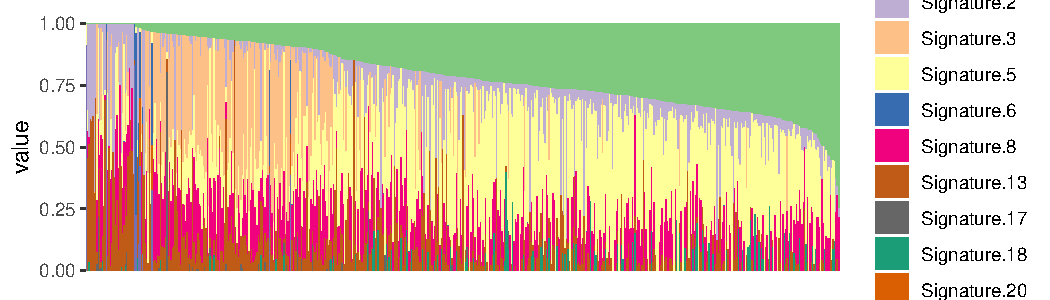
\includegraphics[width=\maxwidth]{figure/unnamed-chunk-8-1} 

\end{knitrout}


\section{Create a \texttt{CompSign} object}
This is a minimal example for transforming a matrix into a \emph{sign} object
\begin{knitrout}
\definecolor{shadecolor}{rgb}{0.969, 0.969, 0.969}\color{fgcolor}\begin{kframe}
\begin{alltt}
\hlstd{basic_matrix} \hlkwb{<-} \hlkwd{matrix}\hlstd{(}\hlkwd{runif}\hlstd{(}\hlnum{12}\hlstd{),} \hlkwc{nrow} \hlstd{=} \hlnum{4}\hlstd{)}
\hlkwd{colnames}\hlstd{(basic_matrix)} \hlkwb{<-} \hlkwd{paste0}\hlstd{(}\hlstr{'s'}\hlstd{,} \hlnum{1}\hlopt{:}\hlnum{3}\hlstd{)}
\hlkwd{rownames}\hlstd{(basic_matrix)} \hlkwb{<-} \hlkwd{paste0}\hlstd{(}\hlstr{'Sample '}\hlstd{,} \hlnum{1}\hlopt{:}\hlnum{4}\hlstd{)}
\hlstd{basic_sign} \hlkwb{<-} \hlkwd{to_sign}\hlstd{(basic_matrix)}
\hlstd{basic_sign}
\end{alltt}
\begin{verbatim}
## An object of class "sign"
## Slot "id":
## [1] "basic_matrix"
## 
## Slot "id_samples":
## [1] "Sample 1" "Sample 2" "Sample 3" "Sample 4"
## 
## Slot "id_signatures":
## [1] "s1" "s2" "s3"
## 
## Slot "count_matrix":
##                 s1        s2        s3
## Sample 1 0.1191255 0.2755550 0.3405389
## Sample 2 0.3432147 0.7431099 0.5742050
## Sample 3 0.4394857 0.3200496 0.7337152
## Sample 4 0.9333408 0.1272246 0.1070315
## 
## Slot "modified":
## [1] FALSE
\end{verbatim}
\end{kframe}
\end{knitrout}

A \emph{sign} object can be summarised as follows:

\hl{add\_together\_matrix?? what is this?}

\begin{knitrout}
\definecolor{shadecolor}{rgb}{0.969, 0.969, 0.969}\color{fgcolor}\begin{kframe}
\begin{alltt}
\hlstd{results_sumarise} \hlkwb{<-} \hlkwd{summarise}\hlstd{(}\hlkwd{add_together_matrix}\hlstd{(basic_sign))}
\hlstd{results_sumarise}
\end{alltt}
\begin{verbatim}
## $General
## [1] "Object of class sign"
## 
## $`Number of signatures`
## [1] 3
## 
## $`Number of samples`
## [1] 4
## 
## $`Geometric means of signatures`
##        s1        s3        s2 
## 0.3598644 0.3520207 0.3021777 
## 
## $Covariance
##             s1          s2          s3
## s1  0.11810025 -0.04176255 -0.04846927
## s2 -0.04176255  0.06983879  0.04187211
## s3 -0.04846927  0.04187211  0.07501169
\end{verbatim}
\end{kframe}
\end{knitrout}

\clearpage
\section{Battery of tests}
This section takes largely from Aitchison's pioneering work\cite{aitchison1982statistical} and its succession\cite{pawlowsky2015modeling}.

\subsection{Test for normality}
\begin{knitrout}
\definecolor{shadecolor}{rgb}{0.969, 0.969, 0.969}\color{fgcolor}\begin{kframe}
\begin{alltt}
\hlkwd{par}\hlstd{(}\hlkwc{mfrow}\hlstd{=}\hlkwd{c}\hlstd{(}\hlnum{1}\hlstd{,}\hlnum{2}\hlstd{))}
\hlkwd{qqnorm.acomp}\hlstd{(}\hlkwd{acomp}\hlstd{(two_normal_pops}\hlopt{@}\hlkwc{count_matrix}\hlstd{),} \hlkwc{pch}\hlstd{=}\hlnum{19}\hlstd{,} \hlkwc{cex}\hlstd{=}\hlnum{0.2}\hlstd{)}
\end{alltt}
\end{kframe}
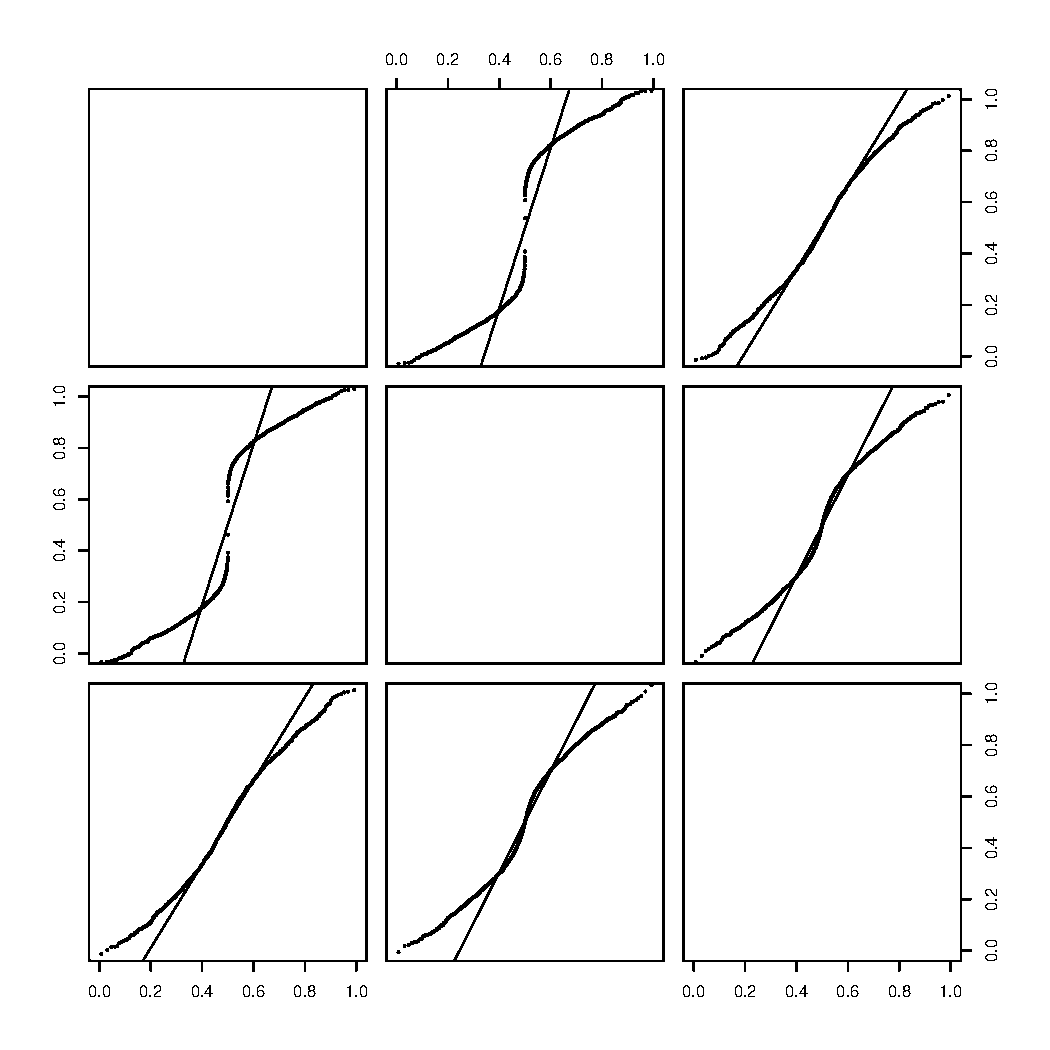
\includegraphics[width=\maxwidth]{figure/unnamed-chunk-11-1} 
\begin{kframe}\begin{alltt}
\hlkwd{qqnorm.acomp}\hlstd{(}\hlkwd{acomp}\hlstd{(two_normal_pops}\hlopt{@}\hlkwc{count_matrix}\hlstd{[}\hlnum{1}\hlopt{:}\hlnum{1000}\hlstd{,]),} \hlkwc{pch}\hlstd{=}\hlnum{19}\hlstd{,} \hlkwc{cex}\hlstd{=}\hlnum{0.2}\hlstd{,} \hlkwc{plot.it}\hlstd{=}\hlnum{FALSE}\hlstd{)}
\end{alltt}


{\ttfamily\noindent\color{warningcolor}{\#\# Warning in plot.window(...): "{}plot.it"{} is not a graphical parameter}}

{\ttfamily\noindent\color{warningcolor}{\#\# Warning in plot.xy(xy, type, ...): "{}plot.it"{} is not a graphical parameter}}

{\ttfamily\noindent\color{warningcolor}{\#\# Warning in title(...): "{}plot.it"{} is not a graphical parameter}}

{\ttfamily\noindent\color{warningcolor}{\#\# Warning in plot.window(...): "{}plot.it"{} is not a graphical parameter}}

{\ttfamily\noindent\color{warningcolor}{\#\# Warning in plot.xy(xy, type, ...): "{}plot.it"{} is not a graphical parameter}}

{\ttfamily\noindent\color{warningcolor}{\#\# Warning in title(...): "{}plot.it"{} is not a graphical parameter}}

{\ttfamily\noindent\color{warningcolor}{\#\# Warning in axis(side = side, at = at, labels = labels, ...): "{}plot.it"{} is not a graphical parameter}}

{\ttfamily\noindent\color{warningcolor}{\#\# Warning in plot.xy(xy.coords(x, y), type = type, ...): "{}plot.it"{} is not a graphical parameter}}

{\ttfamily\noindent\color{warningcolor}{\#\# Warning in plot.window(...): "{}plot.it"{} is not a graphical parameter}}

{\ttfamily\noindent\color{warningcolor}{\#\# Warning in plot.xy(xy, type, ...): "{}plot.it"{} is not a graphical parameter}}

{\ttfamily\noindent\color{warningcolor}{\#\# Warning in title(...): "{}plot.it"{} is not a graphical parameter}}

{\ttfamily\noindent\color{warningcolor}{\#\# Warning in axis(side = side, at = at, labels = labels, ...): "{}plot.it"{} is not a graphical parameter}}

{\ttfamily\noindent\color{warningcolor}{\#\# Warning in plot.xy(xy.coords(x, y), type = type, ...): "{}plot.it"{} is not a graphical parameter}}

{\ttfamily\noindent\color{warningcolor}{\#\# Warning in plot.window(...): "{}plot.it"{} is not a graphical parameter}}

{\ttfamily\noindent\color{warningcolor}{\#\# Warning in plot.xy(xy, type, ...): "{}plot.it"{} is not a graphical parameter}}

{\ttfamily\noindent\color{warningcolor}{\#\# Warning in title(...): "{}plot.it"{} is not a graphical parameter}}

{\ttfamily\noindent\color{warningcolor}{\#\# Warning in axis(side = side, at = at, labels = labels, ...): "{}plot.it"{} is not a graphical parameter}}

{\ttfamily\noindent\color{warningcolor}{\#\# Warning in plot.xy(xy.coords(x, y), type = type, ...): "{}plot.it"{} is not a graphical parameter}}

{\ttfamily\noindent\color{warningcolor}{\#\# Warning in plot.window(...): "{}plot.it"{} is not a graphical parameter}}

{\ttfamily\noindent\color{warningcolor}{\#\# Warning in plot.xy(xy, type, ...): "{}plot.it"{} is not a graphical parameter}}

{\ttfamily\noindent\color{warningcolor}{\#\# Warning in title(...): "{}plot.it"{} is not a graphical parameter}}

{\ttfamily\noindent\color{warningcolor}{\#\# Warning in plot.window(...): "{}plot.it"{} is not a graphical parameter}}

{\ttfamily\noindent\color{warningcolor}{\#\# Warning in plot.xy(xy, type, ...): "{}plot.it"{} is not a graphical parameter}}

{\ttfamily\noindent\color{warningcolor}{\#\# Warning in title(...): "{}plot.it"{} is not a graphical parameter}}

{\ttfamily\noindent\color{warningcolor}{\#\# Warning in plot.xy(xy.coords(x, y), type = type, ...): "{}plot.it"{} is not a graphical parameter}}

{\ttfamily\noindent\color{warningcolor}{\#\# Warning in plot.window(...): "{}plot.it"{} is not a graphical parameter}}

{\ttfamily\noindent\color{warningcolor}{\#\# Warning in plot.xy(xy, type, ...): "{}plot.it"{} is not a graphical parameter}}

{\ttfamily\noindent\color{warningcolor}{\#\# Warning in title(...): "{}plot.it"{} is not a graphical parameter}}

{\ttfamily\noindent\color{warningcolor}{\#\# Warning in axis(side = side, at = at, labels = labels, ...): "{}plot.it"{} is not a graphical parameter}}

{\ttfamily\noindent\color{warningcolor}{\#\# Warning in plot.xy(xy.coords(x, y), type = type, ...): "{}plot.it"{} is not a graphical parameter}}

{\ttfamily\noindent\color{warningcolor}{\#\# Warning in plot.window(...): "{}plot.it"{} is not a graphical parameter}}

{\ttfamily\noindent\color{warningcolor}{\#\# Warning in plot.xy(xy, type, ...): "{}plot.it"{} is not a graphical parameter}}

{\ttfamily\noindent\color{warningcolor}{\#\# Warning in title(...): "{}plot.it"{} is not a graphical parameter}}

{\ttfamily\noindent\color{warningcolor}{\#\# Warning in plot.xy(xy.coords(x, y), type = type, ...): "{}plot.it"{} is not a graphical parameter}}

{\ttfamily\noindent\color{warningcolor}{\#\# Warning in plot.window(...): "{}plot.it"{} is not a graphical parameter}}

{\ttfamily\noindent\color{warningcolor}{\#\# Warning in plot.xy(xy, type, ...): "{}plot.it"{} is not a graphical parameter}}

{\ttfamily\noindent\color{warningcolor}{\#\# Warning in title(...): "{}plot.it"{} is not a graphical parameter}}

{\ttfamily\noindent\color{warningcolor}{\#\# Warning in axis(side = side, at = at, labels = labels, ...): "{}plot.it"{} is not a graphical parameter}}

{\ttfamily\noindent\color{warningcolor}{\#\# Warning in axis(side = side, at = at, labels = labels, ...): "{}plot.it"{} is not a graphical parameter}}\end{kframe}
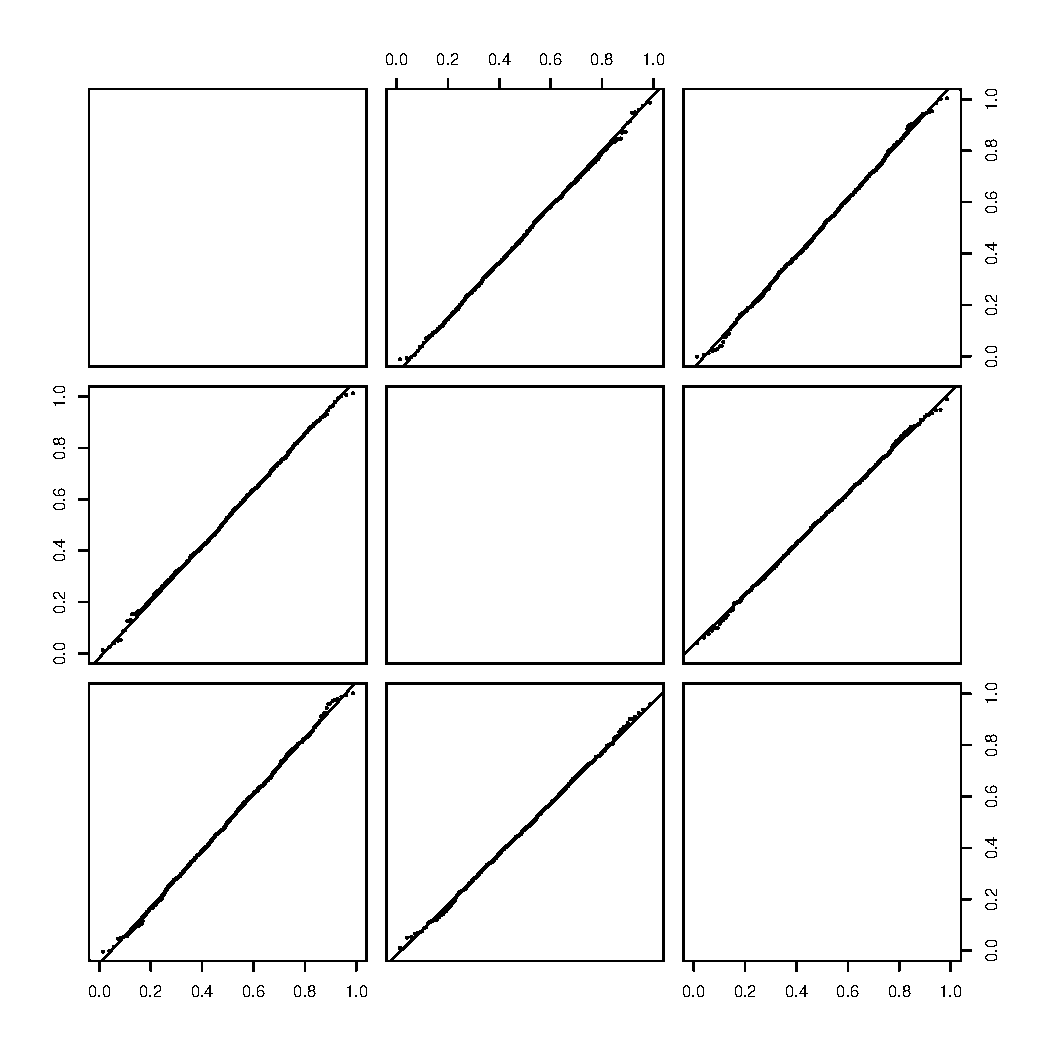
\includegraphics[width=\maxwidth]{figure/unnamed-chunk-11-2} 

\end{knitrout}

\subsection{Test for equality}
Test for equality of means.
\begin{knitrout}
\definecolor{shadecolor}{rgb}{0.969, 0.969, 0.969}\color{fgcolor}\begin{kframe}
\begin{alltt}
\hlkwd{compare_populations}\hlstd{(}\hlkwc{predictors} \hlstd{=} \hlkwd{count_matrix}\hlstd{(Breast560),}
                    \hlkwc{response} \hlstd{=} \hlkwd{as.numeric}\hlstd{(}\hlkwd{as.factor}\hlstd{(}\hlkwd{metadata}\hlstd{(Breast560)}\hlopt{$}\hlstd{final.ER)))}
\end{alltt}
\begin{verbatim}
## $note
## [1] "James test"
## 
## $mesoi
##                  X1         X2       X3           X4        X5       X6
## Sample 1 -1.6969917 -0.9470633 1.923296 -0.103998542 0.2707288 1.528197
## Sample 2  0.8022291 -3.6033765 2.143807  0.002721535 0.6369184 1.607875
##                X7       X8       X9      X10
## Sample 1 1.271388 1.248926 1.016479 1.017358
## Sample 2 1.086473 1.283400 1.083742 1.048809
## 
## $info
##               test            p-value         correction 
##       2.359067e+02       5.324172e-43       1.042820e+00 
## corrected.critical 
##       1.909095e+01
\end{verbatim}
\end{kframe}
\end{knitrout}





\section{Clustering of samples}
Samples can simply be clustered by the cosine similarity of their exposures, as done in Ren et al.

\begin{knitrout}
\definecolor{shadecolor}{rgb}{0.969, 0.969, 0.969}\color{fgcolor}\begin{kframe}
\begin{alltt}
\hlkwd{outerCosineSimilarity}\hlstd{(Breast560, Breast560,} \hlkwc{verbose}\hlstd{=}\hlnum{FALSE}\hlstd{)}
\end{alltt}


{\ttfamily\noindent\bfseries\color{errorcolor}{\#\# Error in outerCosineSimilarity(Breast560, Breast560, verbose = FALSE): unused argument (verbose = FALSE)}}\end{kframe}
\end{knitrout}

\clearpage

\clearpage
\printbibliography

\clearpage
\section{Session info}
\begin{knitrout}
\definecolor{shadecolor}{rgb}{0.969, 0.969, 0.969}\color{fgcolor}\begin{kframe}
\begin{alltt}
  \hlkwd{sessionInfo}\hlstd{()}
\end{alltt}
\begin{verbatim}
## R version 3.5.1 (2018-07-02)
## Platform: x86_64-apple-darwin15.6.0 (64-bit)
## Running under: macOS  10.14.4
## 
## Matrix products: default
## BLAS: /Library/Frameworks/R.framework/Versions/3.5/Resources/lib/libRblas.0.dylib
## LAPACK: /Library/Frameworks/R.framework/Versions/3.5/Resources/lib/libRlapack.dylib
## 
## locale:
## [1] en_GB.UTF-8/en_GB.UTF-8/en_GB.UTF-8/C/en_GB.UTF-8/en_GB.UTF-8
## 
## attached base packages:
## [1] stats     graphics  grDevices utils     datasets  methods   base     
## 
## other attached packages:
##  [1] Compositional_3.4   RColorBrewer_1.1-2  reshape2_1.4.3     
##  [4] ggthemr_1.1.0       ggplot2_3.1.1       MCMCpack_1.4-4     
##  [7] MASS_7.3-51.4       coda_0.19-2         compositions_1.40-2
## [10] bayesm_3.1-1        energy_1.7-5        robustbase_0.93-4  
## [13] tensorA_0.36.1      CompSign_0.1.0      knitr_1.22         
## 
## loaded via a namespace (and not attached):
##  [1] Rcpp_1.0.1         lattice_0.20-38    assertthat_0.2.1  
##  [4] digest_0.6.18      foreach_1.4.4      R6_2.4.0          
##  [7] plyr_1.8.4         MatrixModels_0.4-1 RcppZiggurat_0.1.5
## [10] stats4_3.5.1       evaluate_0.13      spam_2.2-2        
## [13] highr_0.8          pillar_1.3.1       rlang_0.3.4       
## [16] lazyeval_0.2.2     SparseM_1.77       Matrix_1.2-17     
## [19] labeling_0.3       stringr_1.4.0      emplik_1.0-4.3    
## [22] munsell_0.5.0      compiler_3.5.1     numDeriv_2016.8-1 
## [25] xfun_0.6           pkgconfig_2.0.2    mnormt_1.5-5      
## [28] mcmc_0.9-6         tidyselect_0.2.5   tibble_2.1.1      
## [31] codetools_0.2-16   crayon_1.3.4       dplyr_0.8.0.1     
## [34] withr_2.1.2        grid_3.5.1         gtable_0.3.0      
## [37] magrittr_1.5       scales_1.0.0       Rfast_1.9.3       
## [40] stringi_1.4.3      sn_1.5-3           doParallel_1.0.14 
## [43] boot_1.3-22        iterators_1.0.10   tools_3.5.1       
## [46] glue_1.3.1         DEoptimR_1.0-8     purrr_0.3.2       
## [49] maps_3.3.0         fields_9.7         parallel_3.5.1    
## [52] mixture_1.5        colorspace_1.4-1   dotCall64_1.0-0   
## [55] quantreg_5.38
\end{verbatim}
\end{kframe}
\end{knitrout}



\end{document}

\section{Linear model for numerical predictors}
\begin{knitrout}
\definecolor{shadecolor}{rgb}{0.969, 0.969, 0.969}\color{fgcolor}\begin{kframe}
\begin{alltt}
\hlcom{## This chunk was last ran in}
\hlkwd{timestamp}\hlstd{()}
\end{alltt}
\begin{verbatim}
## ##------ Wed May  1 15:40:54 2019 ------##
\end{verbatim}
\begin{alltt}
\hlstd{tmp_merged_compositional} \hlkwb{<-} \hlkwd{new}\hlstd{(}\hlstr{"merged_compositional"}\hlstd{,}
                                \hlkwc{id}\hlstd{=}\hlstr{'adas'}\hlstd{,}
                                \hlkwc{id_samples}\hlstd{=}\hlkwd{paste0}\hlstd{(}\hlstr{"sam"}\hlstd{,} \hlnum{1}\hlopt{:}\hlnum{30}\hlstd{),}
                                \hlkwc{id_signatures}\hlstd{=} \hlkwd{c}\hlstd{(}\hlstr{'s1'}\hlstd{,} \hlstr{'s2'}\hlstd{,} \hlstr{'s3'}\hlstd{,} \hlstr{'s4'}\hlstd{),} \hlcom{## signature names}
                                \hlkwc{count_matrix}\hlstd{=MCMCpack}\hlopt{::}\hlkwd{rdirichlet}\hlstd{(}\hlnum{30}\hlstd{,} \hlkwd{c}\hlstd{(}\hlnum{1}\hlstd{,}\hlnum{1}\hlstd{,}\hlnum{1}\hlstd{,}\hlnum{1}\hlstd{)),}
                                \hlkwc{df}\hlstd{=}\hlkwd{data.frame}\hlstd{(}\hlkwc{a}\hlstd{=}\hlkwd{sample}\hlstd{(}\hlnum{1}\hlopt{:}\hlnum{1e4}\hlstd{,} \hlnum{30}\hlstd{),} \hlkwc{b}\hlstd{=}\hlkwd{rep}\hlstd{(}\hlnum{10}\hlstd{,} \hlnum{30}\hlstd{)))}
\hlkwd{comp_lm}\hlstd{(tmp_merged_compositional)}
\end{alltt}
\begin{verbatim}
## [[1]]
## Response Y1 :
## 
## Call:
## lm(formula = Y1 ~ as.matrix((x@df)[, indices_predictor]))
## 
## Residuals:
##     Min      1Q  Median      3Q     Max 
## -3.6792 -0.5372  0.4192  0.8920  2.2667 
## 
## Coefficients: (1 not defined because of singularities)
##                                          Estimate Std. Error t value
## (Intercept)                             5.356e-02  5.994e-01   0.089
## as.matrix((x@df)[, indices_predictor])a 6.359e-05  9.924e-05   0.641
## as.matrix((x@df)[, indices_predictor])b        NA         NA      NA
##                                         Pr(>|t|)
## (Intercept)                                0.929
## as.matrix((x@df)[, indices_predictor])a    0.527
## as.matrix((x@df)[, indices_predictor])b       NA
## 
## Residual standard error: 1.602 on 28 degrees of freedom
## Multiple R-squared:  0.01445,	Adjusted R-squared:  -0.02074 
## F-statistic: 0.4106 on 1 and 28 DF,  p-value: 0.5269
## 
## 
## Response Y2 :
## 
## Call:
## lm(formula = Y2 ~ as.matrix((x@df)[, indices_predictor]))
## 
## Residuals:
##      Min       1Q   Median       3Q      Max 
## -2.66622 -0.78687  0.05811  0.65760  2.14189 
## 
## Coefficients: (1 not defined because of singularities)
##                                           Estimate Std. Error t value
## (Intercept)                              6.712e-01  4.470e-01   1.501
## as.matrix((x@df)[, indices_predictor])a -1.058e-04  7.402e-05  -1.429
## as.matrix((x@df)[, indices_predictor])b         NA         NA      NA
##                                         Pr(>|t|)
## (Intercept)                                0.144
## as.matrix((x@df)[, indices_predictor])a    0.164
## as.matrix((x@df)[, indices_predictor])b       NA
## 
## Residual standard error: 1.195 on 28 degrees of freedom
## Multiple R-squared:  0.06801,	Adjusted R-squared:  0.03472 
## F-statistic: 2.043 on 1 and 28 DF,  p-value: 0.1639
## 
## 
## Response Y3 :
## 
## Call:
## lm(formula = Y3 ~ as.matrix((x@df)[, indices_predictor]))
## 
## Residuals:
##     Min      1Q  Median      3Q     Max 
## -4.4017 -1.1024  0.3723  0.8181  2.3505 
## 
## Coefficients: (1 not defined because of singularities)
##                                           Estimate Std. Error t value
## (Intercept)                             -3.326e-02  6.122e-01  -0.054
## as.matrix((x@df)[, indices_predictor])a  5.891e-05  1.014e-04   0.581
## as.matrix((x@df)[, indices_predictor])b         NA         NA      NA
##                                         Pr(>|t|)
## (Intercept)                                0.957
## as.matrix((x@df)[, indices_predictor])a    0.566
## as.matrix((x@df)[, indices_predictor])b       NA
## 
## Residual standard error: 1.637 on 28 degrees of freedom
## Multiple R-squared:  0.01192,	Adjusted R-squared:  -0.02337 
## F-statistic: 0.3377 on 1 and 28 DF,  p-value: 0.5658
\end{verbatim}
\end{kframe}
\end{knitrout}

\section{Importing data}
\begin{knitrout}
\definecolor{shadecolor}{rgb}{0.969, 0.969, 0.969}\color{fgcolor}\begin{kframe}
\begin{alltt}
\hlcom{## This chunk was last ran in}
\hlkwd{timestamp}\hlstd{()}
\end{alltt}
\begin{verbatim}
## ##------ Wed May  1 15:40:54 2019 ------##
\end{verbatim}
\begin{alltt}
\hlkwd{biplot}\hlstd{(}\hlkwd{princomp}\hlstd{(}\hlkwd{acomp}\hlstd{(MCMCpack}\hlopt{::}\hlkwd{rdirichlet}\hlstd{(}\hlnum{30}\hlstd{,} \hlkwd{rep}\hlstd{(}\hlnum{1}\hlstd{,} \hlnum{4}\hlstd{)))))}
\end{alltt}
\end{kframe}
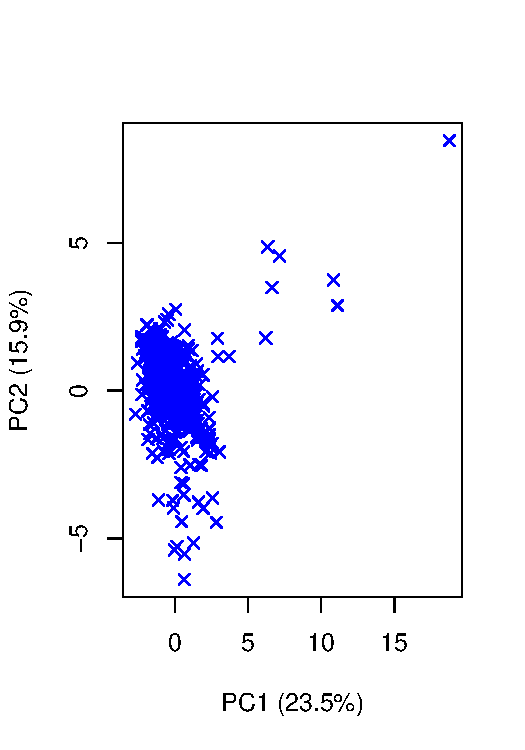
\includegraphics[width=\maxwidth]{figure/unnamed-chunk-17-1} 

\end{knitrout}

\subsection{Testing hypotheses about two populations}
We might have our samples split into two categories; e.g. sex. As in Aithison 1986\cite{}, I follow a hierarchy of alternative hypotheses, from least to most complex.

Our first question is whether two populations have the same covariance and structure and center (i.e. if there is any distributional difference)

\begin{knitrout}
\definecolor{shadecolor}{rgb}{0.969, 0.969, 0.969}\color{fgcolor}\begin{kframe}
\begin{alltt}
\hlcom{## This chunk was last ran in}
\hlkwd{timestamp}\hlstd{()}
\end{alltt}
\begin{verbatim}
## ##------ Wed May  1 15:40:54 2019 ------##
\end{verbatim}
\begin{alltt}
\hlcom{##TODO!!}
\end{alltt}
\end{kframe}
\end{knitrout}

The next is whether the populations have a different center:

\begin{knitrout}
\definecolor{shadecolor}{rgb}{0.969, 0.969, 0.969}\color{fgcolor}\begin{kframe}
\begin{alltt}
\hlcom{## This chunk was last ran in}
\hlkwd{timestamp}\hlstd{()}
\end{alltt}
\begin{verbatim}
## ##------ Wed May  1 15:40:54 2019 ------##
\end{verbatim}
\begin{alltt}
\hlcom{## This dataset includes the two components above, as well as four others}
\hlcom{## (a total of seven)}
\hlkwd{data}\hlstd{(}\hlstr{"two_normal_pops_extended"}\hlstd{)}
\end{alltt}


{\ttfamily\noindent\color{warningcolor}{\#\# Warning in data("{}two\_normal\_pops\_extended"{}): data set 'two\_normal\_pops\_extended' not found}}\begin{alltt}
\hlcom{## Data from the Landscape... paper}
\hlkwd{data}\hlstd{(}\hlstr{"Breast560"}\hlstd{)}
\end{alltt}


{\ttfamily\noindent\color{warningcolor}{\#\# Warning in data("{}Breast560"{}): data set 'Breast560' not found}}\begin{alltt}
\hlstd{wrapper_compare_populations} \hlkwb{<-} \hlkwa{function}\hlstd{(}\hlkwc{predictors}\hlstd{,} \hlkwc{response}\hlstd{,} \hlkwc{...}\hlstd{)\{}
  \hlkwa{if}\hlstd{(}\hlkwd{length}\hlstd{(}\hlkwd{unique}\hlstd{(response))} \hlopt{==} \hlnum{2}\hlstd{)\{}
    \hlstd{tmp} \hlkwb{<-} \hlkwd{compare_populations}\hlstd{(predictors, response, ...)}
    \hlstd{tmp} \hlkwb{<-} \hlstd{tmp}\hlopt{$}\hlstd{info[}\hlnum{1}\hlopt{:}\hlnum{2}\hlstd{]}
    \hlstd{tmp}
  \hlstd{\}}
\hlstd{\}}

\hlstd{x} \hlkwb{<-} \hlkwd{do.call}\hlstd{(}\hlstr{'rbind'}\hlstd{,} \hlkwd{lapply}\hlstd{(}\hlnum{1}\hlopt{:}\hlkwd{ncol}\hlstd{(}\hlkwd{metadata}\hlstd{(Breast560)),}
       \hlkwa{function}\hlstd{(}\hlkwc{k}\hlstd{)\{}
         \hlkwd{wrapper_compare_populations}\hlstd{(}\hlkwc{predictors} \hlstd{=} \hlkwd{count_matrix}\hlstd{(Breast560),}
                                     \hlkwc{response} \hlstd{=} \hlkwd{metadata}\hlstd{(Breast560)[,k])}
         \hlstd{\}}
       \hlstd{))}


\hlstd{x}
\end{alltt}
\begin{verbatim}
##           test      p-value
## [1,] 215.35615 1.224333e-24
## [2,] 161.50152 3.522373e-18
## [3,] 235.90667 5.324172e-43
## [4,]  77.27718 1.042179e-11
\end{verbatim}
\end{kframe}
\end{knitrout}


Not sure if this is correct
\begin{knitrout}
\definecolor{shadecolor}{rgb}{0.969, 0.969, 0.969}\color{fgcolor}\begin{kframe}
\begin{alltt}
\hlkwd{source}\hlstd{(}\hlstr{"../../CDA_in_Cancer/code/functions/basic_functions.R"}\hlstd{)}
\hlkwd{plotPCA}\hlstd{(}\hlkwd{ilr}\hlstd{(}\hlkwd{count_matrix}\hlstd{(Breast560)),} \hlkwc{pch}\hlstd{=}\hlnum{4}\hlstd{,} \hlkwc{col}\hlstd{=}\hlstr{'blue'}\hlstd{)}
\end{alltt}
\end{kframe}
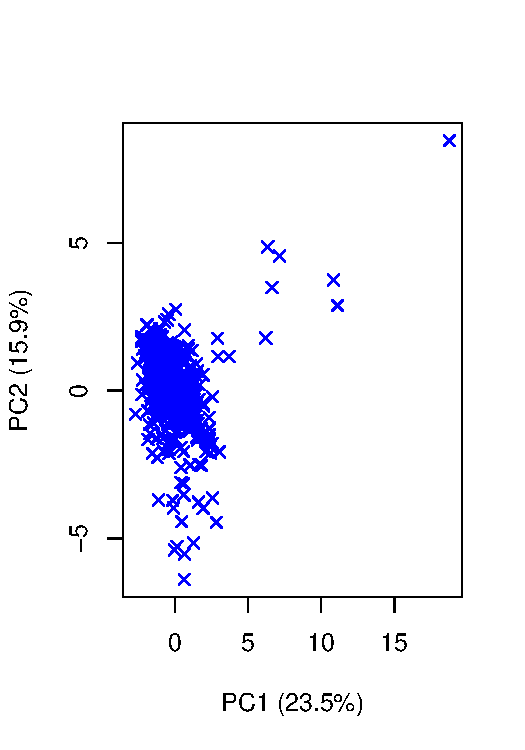
\includegraphics[width=\maxwidth]{figure/unnamed-chunk-20-1} 

\end{knitrout}


\section{Battery of tests}


\subsection{Logistic regression}
Based on ACDWR pg 200

\begin{knitrout}
\definecolor{shadecolor}{rgb}{0.969, 0.969, 0.969}\color{fgcolor}\begin{kframe}
\begin{alltt}
\hlcom{#setwd("~/Documents/PhD/CompSign/vignette_knitr/")}
\hlkwd{load}\hlstd{(}\hlstr{"../data/two_normal_pops_extended.rda"}\hlstd{)}
\hlkwd{load}\hlstd{(}\hlstr{"../data/two_normal_pops_extended.rda"}\hlstd{)}
\hlkwd{load}\hlstd{(}\hlstr{"../data/CNA_12K_TCGA.rda"}\hlstd{)}

\hlcom{## avoid perfect separation}
\hlstd{L} \hlkwb{<-} \hlkwd{length}\hlstd{((}\hlkwd{as.numeric}\hlstd{(}\hlkwd{metadata}\hlstd{(two_normal_pops_extended)[,}\hlnum{1}\hlstd{])))}
\hlstd{scramble} \hlkwb{<-} \hlkwd{sample}\hlstd{(}\hlnum{1}\hlopt{:}\hlstd{L,} \hlkwd{floor}\hlstd{(L}\hlopt{*}\hlnum{0.05}\hlstd{),} \hlkwc{replace} \hlstd{=} \hlnum{FALSE}\hlstd{)}

\hlstd{scrambled_labels} \hlkwb{<-} \hlstd{(}\hlkwd{as.numeric}\hlstd{(}\hlkwd{metadata}\hlstd{(two_normal_pops_extended)[,}\hlnum{1}\hlstd{]))}
\hlstd{scrambled_labels[scramble]} \hlkwb{<-} \hlnum{1}\hlopt{-}\hlstd{scrambled_labels[scramble]}

\hlstd{auxcomp} \hlkwb{<-} \hlkwd{scale}\hlstd{(}\hlkwd{ilr}\hlstd{(}\hlkwd{count_matrix}\hlstd{(two_normal_pops_extended)),}
                 \hlkwc{center} \hlstd{=} \hlnum{TRUE}\hlstd{,} \hlkwc{scale} \hlstd{=} \hlnum{FALSE}\hlstd{)}

\hlkwd{summary}\hlstd{(}\hlkwd{glm}\hlstd{(}\hlkwc{formula} \hlstd{= scrambled_labels} \hlopt{~} \hlkwd{ilr}\hlstd{(}\hlkwd{acomp}\hlstd{(}\hlkwd{count_matrix}\hlstd{(two_normal_pops_extended))),}
            \hlkwc{family} \hlstd{=} \hlkwd{binomial}\hlstd{(}\hlkwc{link} \hlstd{=} \hlstr{"logit"}\hlstd{)))}
\end{alltt}
\begin{verbatim}
## 
## Call:
## glm(formula = scrambled_labels ~ ilr(acomp(count_matrix(two_normal_pops_extended))), 
##     family = binomial(link = "logit"))
## 
## Deviance Residuals: 
##     Min       1Q   Median       3Q      Max  
## -2.8892  -0.3248   0.1483   0.3149   3.0288  
## 
## Coefficients:
##                                                     Estimate Std. Error
## (Intercept)                                          0.49406    0.29857
## ilr(acomp(count_matrix(two_normal_pops_extended)))1  2.13446    0.08000
## ilr(acomp(count_matrix(two_normal_pops_extended)))2 -0.15745    0.20584
## ilr(acomp(count_matrix(two_normal_pops_extended)))3 -0.14823    0.13542
## ilr(acomp(count_matrix(two_normal_pops_extended)))4 -0.07288    0.11831
## ilr(acomp(count_matrix(two_normal_pops_extended)))5 -0.10663    0.10926
## ilr(acomp(count_matrix(two_normal_pops_extended)))6 -0.12304    0.09924
## ilr(acomp(count_matrix(two_normal_pops_extended)))7 -0.09365    0.09904
##                                                     z value Pr(>|z|)    
## (Intercept)                                           1.655    0.098 .  
## ilr(acomp(count_matrix(two_normal_pops_extended)))1  26.682   <2e-16 ***
## ilr(acomp(count_matrix(two_normal_pops_extended)))2  -0.765    0.444    
## ilr(acomp(count_matrix(two_normal_pops_extended)))3  -1.095    0.274    
## ilr(acomp(count_matrix(two_normal_pops_extended)))4  -0.616    0.538    
## ilr(acomp(count_matrix(two_normal_pops_extended)))5  -0.976    0.329    
## ilr(acomp(count_matrix(two_normal_pops_extended)))6  -1.240    0.215    
## ilr(acomp(count_matrix(two_normal_pops_extended)))7  -0.946    0.344    
## ---
## Signif. codes:  0 '***' 0.001 '**' 0.01 '*' 0.05 '.' 0.1 ' ' 1
## 
## (Dispersion parameter for binomial family taken to be 1)
## 
##     Null deviance: 2772.46  on 1999  degrees of freedom
## Residual deviance:  839.68  on 1992  degrees of freedom
## AIC: 855.68
## 
## Number of Fisher Scoring iterations: 6
\end{verbatim}
\begin{alltt}
\hlstd{res} \hlkwb{<-} \hlkwd{comp_logistic}\hlstd{(}\hlkwd{count_matrix}\hlstd{(two_normal_pops), scrambled_labels)}
\end{alltt}


{\ttfamily\noindent\itshape\color{messagecolor}{\#\# Loading required package: nnet}}\begin{verbatim}
## # weights:  5 (4 variable)
## initial  value 1386.294361 
## final  value 443.341841 
## converged
\end{verbatim}
\begin{alltt}
\hlstd{res}
\end{alltt}
\begin{verbatim}
## $coefTransformed
## (Intercept)          X1          X2          X3 
##   0.4036146  -7.0242184   8.1051953  -0.6773624 
## 
## $summary
## Call:
## multinom(formula = as.formula(frm), data = dat)
## 
## Coefficients:
##                 Values Std. Err.
## (Intercept)  0.4036146 0.1363508
## X1          -7.0242184 0.3894933
## X2           8.1051953 0.4014707
## X3          -0.6773624 0.4315879
## 
## Residual Deviance: 886.6837 
## AIC: 892.6837 
## 
## $res
## Call:
## multinom(formula = as.formula(frm), data = dat)
## 
## Coefficients:
## (Intercept)          X1          X2          X3 
##   0.4036146  -7.0242184   8.1051953  -0.6773624 
## 
## Residual Deviance: 886.6837 
## AIC: 892.6837 
## 
## [[4]]
##    FP_FN_table
##       0   1
##   0 946  46
##   1  54 954
\end{verbatim}
\begin{alltt}
\hlstd{resB} \hlkwb{<-} \hlkwd{comp_logistic}\hlstd{(}\hlkwd{count_matrix}\hlstd{(two_normal_pops_extended), scrambled_labels)}
\end{alltt}
\begin{verbatim}
## # weights:  10 (9 variable)
## initial  value 1386.294361 
## final  value 454.019348 
## converged
\end{verbatim}
\begin{alltt}
\hlstd{resB}
\end{alltt}
\begin{verbatim}
## $coefTransformed
##  (Intercept)           X1           X2           X3           X4 
##   0.51686787 -14.25855543  16.15930874  -1.64231937  -0.02158575 
##           X5           X6           X7           X8 
##   0.05490541   0.68247121  -0.67198430   0.21462735 
## 
## $summary
## Call:
## multinom(formula = as.formula(frm), data = dat)
## 
## Coefficients:
##                   Values Std. Err.
## (Intercept)   0.51686787 0.1600932
## X1          -14.25855543 0.7263656
## X2           16.15930874 0.7678407
## X3           -1.64231937 0.8915583
## X4           -0.02158575 0.8961944
## X5            0.05490541 0.8740857
## X6            0.68247121 0.8776382
## X7           -0.67198430 0.9105010
## X8            0.21462735 0.8604837
## 
## Residual Deviance: 908.0387 
## AIC: 922.0387 
## 
## $res
## Call:
## multinom(formula = as.formula(frm), data = dat)
## 
## Coefficients:
##  (Intercept)           X1           X2           X3           X4 
##   0.51686787 -14.25855543  16.15930874  -1.64231937  -0.02158575 
##           X5           X6           X7           X8 
##   0.05490541   0.68247121  -0.67198430   0.21462735 
## 
## Residual Deviance: 908.0387 
## AIC: 922.0387 
## 
## [[4]]
##    FP_FN_table
##       0   1
##   0 946  46
##   1  54 954
\end{verbatim}
\begin{alltt}
\hlstd{resCNA_gender} \hlkwb{<-} \hlkwd{comp_logistic}\hlstd{(}\hlkwd{count_matrix}\hlstd{(}\hlkwd{cleanObject}\hlstd{(CNA_12K_TCGA,} \hlstr{'gender'}\hlstd{)),}
                              \hlkwd{metadata}\hlstd{(}\hlkwd{cleanObject}\hlstd{(CNA_12K_TCGA,} \hlstr{'gender'}\hlstd{))[,}\hlstr{'gender'}\hlstd{])}
\end{alltt}
\begin{verbatim}
## # weights:  9 (8 variable)
## initial  value 7535.896147 
## iter  10 value 7477.896938
## final  value 7477.896342 
## converged
\end{verbatim}
\begin{alltt}
\hlstd{resCNA_gender}
\end{alltt}
\begin{verbatim}
## $coefTransformed
## (Intercept)          s1          s2          s3          s4          s5 
##  -0.2991671   0.2381913  -1.5952762  -0.7137485  -0.3424139   1.1287220 
##          s6          s7 
##   1.1463550  -0.1609969 
## 
## $summary
## Call:
## multinom(formula = as.formula(frm), data = dat)
## 
## Coefficients:
##                 Values  Std. Err.
## (Intercept) -0.2991671 0.04634220
## s1           0.2381913 0.07069156
## s2          -1.5952762 0.34187887
## s3          -0.7137485 0.15918132
## s4          -0.3424139 0.22213187
## s5           1.1287220 0.15577367
## s6           1.1463550 0.25201363
## s7          -0.1609969 0.19798834
## 
## Residual Deviance: 14955.79 
## AIC: 14969.79 
## 
## $res
## Call:
## multinom(formula = as.formula(frm), data = dat)
## 
## Coefficients:
## (Intercept)          s1          s2          s3          s4          s5 
##  -0.2991671   0.2381913  -1.5952762  -0.7137485  -0.3424139   1.1287220 
##          s6          s7 
##   1.1463550  -0.1609969 
## 
## Residual Deviance: 14955.79 
## AIC: 14969.79 
## 
## [[4]]
##         FP_FN_table
##             0    1
##   female 4268 1385
##   male   3520 1699
\end{verbatim}
\begin{alltt}
\hlcom{## below: incorrect}
\hlstd{resCNA_race} \hlkwb{<-} \hlkwd{comp_logistic}\hlstd{(}\hlkwd{count_matrix}\hlstd{(}\hlkwd{cleanObject}\hlstd{(CNA_12K_TCGA,} \hlstr{'race'}\hlstd{)),}
                              \hlkwd{metadata}\hlstd{(}\hlkwd{cleanObject}\hlstd{(CNA_12K_TCGA,} \hlstr{'race'}\hlstd{))[,}\hlstr{'race'}\hlstd{],} \hlkwc{relax_binary_assumption} \hlstd{=} \hlnum{TRUE}\hlstd{)}
\end{alltt}
\begin{verbatim}
## # weights:  45 (32 variable)
## initial  value 15411.977449 
## iter  10 value 5840.051105
## iter  20 value 5603.221335
## iter  30 value 5590.128772
## iter  40 value 5589.864008
## final  value 5589.860769 
## converged
\end{verbatim}
\begin{alltt}
\hlstd{resCNA_race}
\end{alltt}
\begin{verbatim}
## $coefTransformed
##                                           (Intercept)         s1        s2
## asian                                        2.672068  0.9450276 -3.803121
## black or african american                    3.115921  0.7428933 -2.324556
## native hawaiian or other pacific islander   -2.901050 -1.0452138 -6.000538
## white                                        4.861007  1.4719541 -2.635247
##                                                 s3         s4        s5
## asian                                     1.674742 -0.5989746 -1.248396
## black or african american                 2.166487  0.9507823 -2.065123
## native hawaiian or other pacific islander 2.378382  8.4160702  4.209867
## white                                     1.954892  0.1143870 -1.117764
##                                                    s6       s7
## asian                                       1.6917138 4.011077
## black or african american                  -0.0387949 3.684232
## native hawaiian or other pacific islander -12.2816314 1.422015
## white                                       1.0833213 3.989464
## 
## $summary
## Call:
## multinom(formula = as.formula(frm), data = dat)
## 
## Coefficients:
##                                           (Intercept)         s1        s2
## asian                                        2.672068  0.9450276 -3.803121
## black or african american                    3.115921  0.7428933 -2.324556
## native hawaiian or other pacific islander   -2.901050 -1.0452138 -6.000538
## white                                        4.861007  1.4719541 -2.635247
##                                                 s3         s4        s5
## asian                                     1.674742 -0.5989746 -1.248396
## black or african american                 2.166487  0.9507823 -2.065123
## native hawaiian or other pacific islander 2.378382  8.4160702  4.209867
## white                                     1.954892  0.1143870 -1.117764
##                                                    s6       s7
## asian                                       1.6917138 4.011077
## black or african american                  -0.0387949 3.684232
## native hawaiian or other pacific islander -12.2816314 1.422015
## white                                       1.0833213 3.989464
## 
## Std. Errors:
##                                           (Intercept)        s1       s2
## asian                                       0.3673940 0.7296476 2.413953
## black or african american                   0.3615361 0.7244379 2.356048
## native hawaiian or other pacific islander   0.9978657 2.0548757 5.411428
## white                                       0.3555740 0.7157202 2.308680
##                                                 s3       s4       s5
## asian                                     1.493635 2.115974 1.274487
## black or african american                 1.483318 2.095245 1.266690
## native hawaiian or other pacific islander 2.632530 3.047898 2.174688
## white                                     1.461269 2.070342 1.240876
##                                                 s6       s7
## asian                                     2.345331 1.977182
## black or african american                 2.337053 1.966071
## native hawaiian or other pacific islander 5.880740 3.158845
## white                                     2.302844 1.941439
## 
## Residual Deviance: 11179.72 
## AIC: 11235.72 
## 
## $res
## Call:
## multinom(formula = as.formula(frm), data = dat)
## 
## Coefficients:
##                                           (Intercept)         s1        s2
## asian                                        2.672068  0.9450276 -3.803121
## black or african american                    3.115921  0.7428933 -2.324556
## native hawaiian or other pacific islander   -2.901050 -1.0452138 -6.000538
## white                                        4.861007  1.4719541 -2.635247
##                                                 s3         s4        s5
## asian                                     1.674742 -0.5989746 -1.248396
## black or african american                 2.166487  0.9507823 -2.065123
## native hawaiian or other pacific islander 2.378382  8.4160702  4.209867
## white                                     1.954892  0.1143870 -1.117764
##                                                    s6       s7
## asian                                       1.6917138 4.011077
## black or african american                  -0.0387949 3.684232
## native hawaiian or other pacific islander -12.2816314 1.422015
## white                                       1.0833213 3.989464
## 
## Residual Deviance: 11179.72 
## AIC: 11235.72 
## 
## [[4]]
##                                            FP_FN_table
##                                                0
##   american indian or alaska native            27
##   asian                                      665
##   black or african american                  910
##   native hawaiian or other pacific islander   13
##   white                                     7961
\end{verbatim}
\end{kframe}
\end{knitrout}

With data from 560 BRCA:

\begin{knitrout}
\definecolor{shadecolor}{rgb}{0.969, 0.969, 0.969}\color{fgcolor}\begin{kframe}
\begin{alltt}
\hlkwd{load}\hlstd{(}\hlstr{"../data/Breast560.rda"}\hlstd{)}

\hlstd{resBRCA_finalER} \hlkwb{<-} \hlkwd{comp_logistic}\hlstd{(}\hlkwd{count_matrix}\hlstd{(}\hlkwd{cleanObject}\hlstd{(Breast560,} \hlstr{'final.ER'}\hlstd{)),}
                              \hlkwd{metadata}\hlstd{(}\hlkwd{cleanObject}\hlstd{(Breast560,} \hlstr{'final.ER'}\hlstd{))[,}\hlstr{'final.ER'}\hlstd{])}
\end{alltt}
\begin{verbatim}
## # weights:  14 (13 variable)
## initial  value 388.162421 
## iter  10 value 247.760067
## iter  20 value 247.644411
## final  value 247.613009 
## converged
\end{verbatim}
\begin{alltt}
\hlstd{resBRCA_finalER}
\end{alltt}
\begin{verbatim}
## $coefTransformed
##  (Intercept)  Signature.1  Signature.2  Signature.3  Signature.5 
##  -1.37260416   6.87524489   6.08117930  -2.62251433   1.45209910 
##  Signature.6  Signature.8 Signature.13 Signature.17 Signature.18 
##  -4.32588363   1.61674367  -1.28298467  -3.96303199   0.04978287 
## Signature.20 Signature.26 Signature.30 
##  -0.08628501   2.83168183  -7.99863619 
## 
## $summary
## Call:
## multinom(formula = as.formula(frm), data = dat)
## 
## Coefficients:
##                   Values Std. Err.
## (Intercept)  -1.37260416  3.251285
## Signature.1   6.87524489  3.433278
## Signature.2   6.08117930  3.539466
## Signature.3  -2.62251433  3.308807
## Signature.5   1.45209910  3.315171
## Signature.6  -4.32588363  5.520552
## Signature.8   1.61674367  3.367322
## Signature.13 -1.28298467  3.412039
## Signature.17 -3.96303199  5.302369
## Signature.18  0.04978287  3.950056
## Signature.20 -0.08628501  8.963178
## Signature.26  2.83168183  3.620818
## Signature.30 -7.99863619 38.183574
## 
## Residual Deviance: 495.226 
## AIC: 519.226 
## 
## $res
## Call:
## multinom(formula = as.formula(frm), data = dat)
## 
## Coefficients:
##  (Intercept)  Signature.1  Signature.2  Signature.3  Signature.5 
##  -1.37260416   6.87524489   6.08117930  -2.62251433   1.45209910 
##  Signature.6  Signature.8 Signature.13 Signature.17 Signature.18 
##  -4.32588363   1.61674367  -1.28298467  -3.96303199   0.04978287 
## Signature.20 Signature.26 Signature.30 
##  -0.08628501   2.83168183  -7.99863619 
## 
## Residual Deviance: 495.226 
## AIC: 519.226 
## 
## [[4]]
##           FP_FN_table
##              0   1
##   negative 125  69
##   positive  40 326
\end{verbatim}
\begin{alltt}
\hlstd{resBRCA_finalPR} \hlkwb{<-} \hlkwd{comp_logistic}\hlstd{(}\hlkwd{count_matrix}\hlstd{(}\hlkwd{cleanObject}\hlstd{(Breast560,} \hlstr{'final.PR'}\hlstd{)),}
                                 \hlkwd{metadata}\hlstd{(}\hlkwd{cleanObject}\hlstd{(Breast560,} \hlstr{'final.PR'}\hlstd{))[,}\hlstr{'final.PR'}\hlstd{])}
\end{alltt}
\begin{verbatim}
## # weights:  14 (13 variable)
## initial  value 381.924096 
## iter  10 value 286.749871
## iter  20 value 286.622284
## iter  30 value 286.593699
## iter  40 value 286.591998
## iter  50 value 286.591708
## iter  60 value 286.590956
## final  value 286.590900 
## converged
\end{verbatim}
\begin{alltt}
\hlstd{resBRCA_finalPR}
\end{alltt}
\begin{verbatim}
## $coefTransformed
##  (Intercept)  Signature.1  Signature.2  Signature.3  Signature.5 
## -2.153476504  6.447772998  4.352131758 -1.669248002  2.473918774 
##  Signature.6  Signature.8 Signature.13 Signature.17 Signature.18 
## -2.429820875  1.398766627 -0.003181878 -2.594728791 -3.577849924 
## Signature.20 Signature.26 Signature.30 
## -0.411942687  3.502727024 -9.642021527 
## 
## $summary
## Call:
## multinom(formula = as.formula(frm), data = dat)
## 
## Coefficients:
##                    Values Std. Err.
## (Intercept)  -2.153476504  5.783443
## Signature.1   6.447772998  5.857258
## Signature.2   4.352131758  5.887041
## Signature.3  -1.669248002  5.816657
## Signature.5   2.473918774  5.810631
## Signature.6  -2.429820875  7.009770
## Signature.8   1.398766627  5.841518
## Signature.13 -0.003181878  5.856845
## Signature.17 -2.594728791  7.104266
## Signature.18 -3.577849924  6.084505
## Signature.20 -0.411942687  9.928254
## Signature.26  3.502727024  5.991856
## Signature.30 -9.642021527 68.949229
## 
## Residual Deviance: 573.1818 
## AIC: 597.1818 
## 
## $res
## Call:
## multinom(formula = as.formula(frm), data = dat)
## 
## Coefficients:
##  (Intercept)  Signature.1  Signature.2  Signature.3  Signature.5 
## -2.153476504  6.447772998  4.352131758 -1.669248002  2.473918774 
##  Signature.6  Signature.8 Signature.13 Signature.17 Signature.18 
## -2.429820875  1.398766627 -0.003181878 -2.594728791 -3.577849924 
## Signature.20 Signature.26 Signature.30 
## -0.411942687  3.502727024 -9.642021527 
## 
## Residual Deviance: 573.1818 
## AIC: 597.1818 
## 
## [[4]]
##           FP_FN_table
##              0   1
##   negative 146  92
##   positive  49 264
\end{verbatim}
\end{kframe}
\end{knitrout}

How to get p-values? I don't think the below is correct
\begin{knitrout}
\definecolor{shadecolor}{rgb}{0.969, 0.969, 0.969}\color{fgcolor}\begin{kframe}
\begin{alltt}
\hlstd{give_pval} \hlkwb{<-} \hlkwa{function}\hlstd{(}\hlkwc{summary_obj}\hlstd{)\{}
  \hlstd{z} \hlkwb{<-} \hlstd{summary_obj}\hlopt{$}\hlstd{coefficients}\hlopt{/}\hlstd{summary_obj}\hlopt{$}\hlstd{standard.errors}
  \hlcom{# 2-tailed Wald z tests to test significance of coefficients}
  \hlstd{p} \hlkwb{<-} \hlstd{(}\hlnum{1} \hlopt{-} \hlkwd{pnorm}\hlstd{(}\hlkwd{abs}\hlstd{(z),} \hlnum{0}\hlstd{,} \hlnum{1}\hlstd{))} \hlopt{*} \hlnum{2}
  \hlstd{p}
\hlstd{\}}

\hlkwd{give_pval}\hlstd{(res}\hlopt{$}\hlstd{summary)}             \hlcom{## 1 and two are; the third one too (higher p-val) (third one wasn't expected, as far as I know?)}
\end{alltt}
\begin{verbatim}
## (Intercept)          X1          X2          X3 
## 0.003075197 0.000000000 0.000000000 0.116539511
\end{verbatim}
\begin{alltt}
\hlkwd{give_pval}\hlstd{(resB}\hlopt{$}\hlstd{summary)}            \hlcom{## 1 and two are; the rest are not (as expected)}
\end{alltt}
\begin{verbatim}
## (Intercept)          X1          X2          X3          X4          X5 
## 0.001244227 0.000000000 0.000000000 0.065463845 0.980784000 0.949914077 
##          X6          X7          X8 
## 0.436791603 0.460491378 0.803030968
\end{verbatim}
\begin{alltt}
\hlkwd{give_pval}\hlstd{(resCNA_gender}\hlopt{$}\hlstd{summary)}   \hlcom{## are are statistically significant for the copy number signatures}
\end{alltt}
\begin{verbatim}
##  (Intercept)           s1           s2           s3           s4 
## 1.077847e-10 7.531978e-04 3.068168e-06 7.330097e-06 1.231978e-01 
##           s5           s6           s7 
## 4.294343e-13 5.395732e-06 4.161242e-01
\end{verbatim}
\begin{alltt}
\hlkwd{give_pval}\hlstd{(resBRCA_finalER}\hlopt{$}\hlstd{summary)} \hlcom{## signature 1 significant}
\end{alltt}
\begin{verbatim}
##  (Intercept)  Signature.1  Signature.2  Signature.3  Signature.5 
##   0.67289887   0.04522767   0.08577724   0.42801901   0.66137441 
##  Signature.6  Signature.8 Signature.13 Signature.17 Signature.18 
##   0.43327710   0.63113682   0.70690426   0.45481743   0.98994446 
## Signature.20 Signature.26 Signature.30 
##   0.99231920   0.43418178   0.83407475
\end{verbatim}
\begin{alltt}
\hlkwd{give_pval}\hlstd{(resBRCA_finalPR}\hlopt{$}\hlstd{summary)} \hlcom{## none are statistically significant}
\end{alltt}
\begin{verbatim}
##  (Intercept)  Signature.1  Signature.2  Signature.3  Signature.5 
##    0.7096308    0.2709760    0.4597411    0.7741298    0.6702847 
##  Signature.6  Signature.8 Signature.13 Signature.17 Signature.18 
##    0.7288667    0.8107547    0.9995665    0.7149358    0.5565145 
## Signature.20 Signature.26 Signature.30 
##    0.9669037    0.5588293    0.8887846
\end{verbatim}
\begin{alltt}
\hlkwd{give_pval}\hlstd{(resCNA_race}\hlopt{$}\hlstd{summary)}     \hlcom{## some statistically significant}
\end{alltt}
\begin{verbatim}
##                                            (Intercept)         s1
## asian                                     3.514966e-13 0.19525689
## black or african american                 0.000000e+00 0.30513893
## native hawaiian or other pacific islander 3.646162e-03 0.61099712
## white                                     0.000000e+00 0.03972419
##                                                  s2        s3          s4
## asian                                     0.1151469 0.2621805 0.777121091
## black or african american                 0.3238222 0.1441339 0.649986482
## native hawaiian or other pacific islander 0.2674888 0.3662825 0.005757702
## white                                     0.2536819 0.1809603 0.955939057
##                                                   s5         s6         s7
## asian                                     0.32731885 0.47071795 0.04249054
## black or african american                 0.10303171 0.98675579 0.06094340
## native hawaiian or other pacific islander 0.05288625 0.03675726 0.65258836
## white                                     0.36770184 0.63804960 0.03988860
\end{verbatim}
\end{kframe}
\end{knitrout}

\begin{knitrout}
\definecolor{shadecolor}{rgb}{0.969, 0.969, 0.969}\color{fgcolor}\begin{kframe}
\begin{alltt}
\hlstd{wrapper_single_logReg} \hlkwb{<-} \hlkwa{function}\hlstd{(}\hlkwc{colname}\hlstd{,} \hlkwc{Ddd}\hlstd{)\{}
    \hlkwd{print}\hlstd{(}\hlstr{'asdsd2'}\hlstd{)}
    \hlkwd{print}\hlstd{(}\hlkwd{head}\hlstd{(}\hlkwd{metadata}\hlstd{((Ddd))))}
    \hlstd{Ddd} \hlkwb{<-} \hlkwd{cleanObject}\hlstd{(Ddd, colname)}
    \hlstd{compData} \hlkwb{=} \hlkwd{count_matrix}\hlstd{(Ddd)}
    \hlstd{binaryLabels} \hlkwb{=} \hlkwd{metadata}\hlstd{(Ddd)[,colname]}

    \hlstd{tmp} \hlkwb{<-} \hlkwd{comp_logistic}\hlstd{(}\hlkwc{compData} \hlstd{= compData,}
                         \hlkwc{binaryLabels} \hlstd{= binaryLabels,}
                         \hlkwc{relax_binary_assumption} \hlstd{=} \hlnum{TRUE}\hlstd{)}
\hlcom{#    give_pval(tmp$summary)}
    \hlkwd{print}\hlstd{(}\hlkwd{give_pval}\hlstd{(tmp}\hlopt{$}\hlstd{summary))}
    \hlkwd{cbind.data.frame}\hlstd{(}\hlkwd{rep}\hlstd{(colname,} \hlkwd{nrow}\hlstd{(} \hlkwd{give_pval}\hlstd{(tmp}\hlopt{$}\hlstd{summary))),} \hlkwd{give_pval}\hlstd{(tmp}\hlopt{$}\hlstd{summary))}
    \hlkwd{cbind.data.frame}\hlstd{(}\hlkwd{rep}\hlstd{(colname,} \hlkwd{nrow}\hlstd{(} \hlkwd{give_pval}\hlstd{(tmp}\hlopt{$}\hlstd{summary))),} \hlkwd{give_pval}\hlstd{(tmp}\hlopt{$}\hlstd{summary))}
\hlstd{\}}
\hlstd{wrapper_multiple_logReg} \hlkwb{<-} \hlkwa{function}\hlstd{(}\hlkwc{dataset}\hlstd{,} \hlkwc{colnames}\hlstd{)\{}
  \hlkwd{print}\hlstd{(}\hlstr{'asdsd'}\hlstd{)}
  \hlkwd{head}\hlstd{(}\hlkwd{metadata}\hlstd{(dataset))}
  \hlkwd{do.call}\hlstd{(}\hlstr{'rbind'}\hlstd{,} \hlkwd{lapply}\hlstd{(colnames,} \hlkwa{function}\hlstd{(}\hlkwc{X}\hlstd{)} \hlkwd{wrapper_single_logReg}\hlstd{(}\hlkwc{colname} \hlstd{= X,} \hlkwc{Ddd} \hlstd{= dataset)))}
\hlstd{\}}

\hlkwd{wrapper_single_logReg}\hlstd{(}\hlstr{'race'}\hlstd{, CNA_12K_TCGA)}
\end{alltt}
\begin{verbatim}
## [1] "asdsd2"
##                                case_id submitter_id project_id gender
## 1 3144f1fb-4342-4079-bfe8-940da4bfd88e TCGA-E2-A14V  TCGA-BRCA female
## 2 4922cddc-575c-4b8a-8245-ce5f6876760c TCGA-E9-A1R3  TCGA-BRCA female
## 3 b0f8d698-a30e-4d8d-b0a2-a5a01fac8406 TCGA-A2-A0T4  TCGA-BRCA female
## 4 2b36853f-34d3-47c5-ba6a-e5a93233d2b1 TCGA-AC-A7VC  TCGA-BRCA female
## 5 8c7e74e0-71ef-49b8-9217-94b8ef740ef9 TCGA-A7-A13E  TCGA-BRCA female
## 6 bfa3dbc0-361c-400e-8c10-0aca7049fce9 TCGA-D8-A27W  TCGA-BRCA female
##   year_of_birth  race              ethnicity year_of_death
## 1          1955 white not hispanic or latino            --
## 2          1940 white not hispanic or latino            --
## 3          1947 white not hispanic or latino            --
## 4          1957 white not hispanic or latino            --
## 5          1948 white not hispanic or latino            --
## 6          1956 white not hispanic or latino            --
##   classification_of_tumor last_known_disease_status
## 1            not reported              not reported
## 2            not reported              not reported
## 3            not reported              not reported
## 4            not reported              not reported
## 5            not reported              not reported
## 6            not reported              not reported
##                  primary_diagnosis tumor_stage age_at_diagnosis
## 1 Infiltrating duct carcinoma, NOS   stage iib            19643
## 2 Infiltrating duct carcinoma, NOS  stage iiic            25693
## 3           Lobular carcinoma, NOS   stage iia            22849
## 4       Metaplastic carcinoma, NOS   stage iib            20479
## 5 Infiltrating duct carcinoma, NOS   stage iib            22690
## 6          Mucinous adenocarcinoma  stage iiib            20173
##   vital_status morphology days_to_death days_to_last_known_disease_status
## 1        alive     8500/3            --                                --
## 2        alive     8500/3            --                                --
## 3        alive     8520/3            --                                --
## 4        alive     8575/3            --                                --
## 5         dead     8500/3         614.0                                --
## 6        alive     8480/3            --                                --
##   days_to_recurrence  tumor_grade tissue_or_organ_of_origin days_to_birth
## 1                 -- not reported               Breast, NOS      -19643.0
## 2                 -- not reported               Breast, NOS      -25693.0
## 3                 -- not reported               Breast, NOS      -22849.0
## 4                 -- not reported               Breast, NOS      -20479.0
## 5                 -- not reported               Breast, NOS      -22690.0
## 6                 -- not reported               Breast, NOS      -20173.0
##   progression_or_recurrence prior_malignancy site_of_resection_or_biopsy
## 1              not reported     not reported                 Breast, NOS
## 2              not reported     not reported                 Breast, NOS
## 3              not reported     not reported                 Breast, NOS
## 4              not reported     not reported                 Breast, NOS
## 5              not reported     not reported                 Breast, NOS
## 6              not reported     not reported                 Breast, NOS
##   days_to_last_follow_up therapeutic_agents treatment_intent_type
## 1                 1042.0                 --                    --
## 2                   78.0                 --                    --
## 3                  624.0                 --                    --
## 4                    1.0                 --                    --
## 5                  326.0                 --                    --
## 6                  373.0                 --                    --
##   treatment_or_therapy submitter_id project_id cigarettes_per_day weight
## 1                   -- TCGA-E2-A14V  TCGA-BRCA                 --     --
## 2                   -- TCGA-E9-A1R3  TCGA-BRCA                 --     --
## 3                   -- TCGA-A2-A0T4  TCGA-BRCA                 --     --
## 4                   -- TCGA-AC-A7VC  TCGA-BRCA                 --     --
## 5                   -- TCGA-A7-A13E  TCGA-BRCA                 --     --
## 6                   -- TCGA-D8-A27W  TCGA-BRCA                 --     --
##   alcohol_history alcohol_intensity bmi years_smoked height
## 1              --                --  --           --     --
## 2              --                --  --           --     --
## 3              --                --  --           --     --
## 4              --                --  --           --     --
## 5              --                --  --           --     --
## 6              --                --  --           --     --
## # weights:  45 (32 variable)
## initial  value 15411.977449 
## iter  10 value 5840.051105
## iter  20 value 5603.221335
## iter  30 value 5590.128772
## iter  40 value 5589.864008
## final  value 5589.860769 
## converged
##                                            (Intercept)         s1
## asian                                     3.514966e-13 0.19525689
## black or african american                 0.000000e+00 0.30513893
## native hawaiian or other pacific islander 3.646162e-03 0.61099712
## white                                     0.000000e+00 0.03972419
##                                                  s2        s3          s4
## asian                                     0.1151469 0.2621805 0.777121091
## black or african american                 0.3238222 0.1441339 0.649986482
## native hawaiian or other pacific islander 0.2674888 0.3662825 0.005757702
## white                                     0.2536819 0.1809603 0.955939057
##                                                   s5         s6         s7
## asian                                     0.32731885 0.47071795 0.04249054
## black or african american                 0.10303171 0.98675579 0.06094340
## native hawaiian or other pacific islander 0.05288625 0.03675726 0.65258836
## white                                     0.36770184 0.63804960 0.03988860
##                                           rep(colname, nrow(give_pval(tmp$summary)))
## asian                                                                           race
## black or african american                                                       race
## native hawaiian or other pacific islander                                       race
## white                                                                           race
##                                            (Intercept)         s1
## asian                                     3.514966e-13 0.19525689
## black or african american                 0.000000e+00 0.30513893
## native hawaiian or other pacific islander 3.646162e-03 0.61099712
## white                                     0.000000e+00 0.03972419
##                                                  s2        s3          s4
## asian                                     0.1151469 0.2621805 0.777121091
## black or african american                 0.3238222 0.1441339 0.649986482
## native hawaiian or other pacific islander 0.2674888 0.3662825 0.005757702
## white                                     0.2536819 0.1809603 0.955939057
##                                                   s5         s6         s7
## asian                                     0.32731885 0.47071795 0.04249054
## black or african american                 0.10303171 0.98675579 0.06094340
## native hawaiian or other pacific islander 0.05288625 0.03675726 0.65258836
## white                                     0.36770184 0.63804960 0.03988860
\end{verbatim}
\begin{alltt}
\hlstd{all_cna} \hlkwb{<-} \hlkwd{wrapper_multiple_logReg}\hlstd{(}\hlkwc{dataset} \hlstd{= CNA_12K_TCGA,}
                                 \hlkwc{colnames} \hlstd{=} \hlkwd{c}\hlstd{(}\hlstr{'race'}\hlstd{,} \hlstr{'ethnicity'}\hlstd{,} \hlstr{'gender'}\hlstd{,} \hlstr{'alcohol_history'}\hlstd{))}
\end{alltt}
\begin{verbatim}
## [1] "asdsd"
## [1] "asdsd2"
##                                case_id submitter_id project_id gender
## 1 3144f1fb-4342-4079-bfe8-940da4bfd88e TCGA-E2-A14V  TCGA-BRCA female
## 2 4922cddc-575c-4b8a-8245-ce5f6876760c TCGA-E9-A1R3  TCGA-BRCA female
## 3 b0f8d698-a30e-4d8d-b0a2-a5a01fac8406 TCGA-A2-A0T4  TCGA-BRCA female
## 4 2b36853f-34d3-47c5-ba6a-e5a93233d2b1 TCGA-AC-A7VC  TCGA-BRCA female
## 5 8c7e74e0-71ef-49b8-9217-94b8ef740ef9 TCGA-A7-A13E  TCGA-BRCA female
## 6 bfa3dbc0-361c-400e-8c10-0aca7049fce9 TCGA-D8-A27W  TCGA-BRCA female
##   year_of_birth  race              ethnicity year_of_death
## 1          1955 white not hispanic or latino            --
## 2          1940 white not hispanic or latino            --
## 3          1947 white not hispanic or latino            --
## 4          1957 white not hispanic or latino            --
## 5          1948 white not hispanic or latino            --
## 6          1956 white not hispanic or latino            --
##   classification_of_tumor last_known_disease_status
## 1            not reported              not reported
## 2            not reported              not reported
## 3            not reported              not reported
## 4            not reported              not reported
## 5            not reported              not reported
## 6            not reported              not reported
##                  primary_diagnosis tumor_stage age_at_diagnosis
## 1 Infiltrating duct carcinoma, NOS   stage iib            19643
## 2 Infiltrating duct carcinoma, NOS  stage iiic            25693
## 3           Lobular carcinoma, NOS   stage iia            22849
## 4       Metaplastic carcinoma, NOS   stage iib            20479
## 5 Infiltrating duct carcinoma, NOS   stage iib            22690
## 6          Mucinous adenocarcinoma  stage iiib            20173
##   vital_status morphology days_to_death days_to_last_known_disease_status
## 1        alive     8500/3            --                                --
## 2        alive     8500/3            --                                --
## 3        alive     8520/3            --                                --
## 4        alive     8575/3            --                                --
## 5         dead     8500/3         614.0                                --
## 6        alive     8480/3            --                                --
##   days_to_recurrence  tumor_grade tissue_or_organ_of_origin days_to_birth
## 1                 -- not reported               Breast, NOS      -19643.0
## 2                 -- not reported               Breast, NOS      -25693.0
## 3                 -- not reported               Breast, NOS      -22849.0
## 4                 -- not reported               Breast, NOS      -20479.0
## 5                 -- not reported               Breast, NOS      -22690.0
## 6                 -- not reported               Breast, NOS      -20173.0
##   progression_or_recurrence prior_malignancy site_of_resection_or_biopsy
## 1              not reported     not reported                 Breast, NOS
## 2              not reported     not reported                 Breast, NOS
## 3              not reported     not reported                 Breast, NOS
## 4              not reported     not reported                 Breast, NOS
## 5              not reported     not reported                 Breast, NOS
## 6              not reported     not reported                 Breast, NOS
##   days_to_last_follow_up therapeutic_agents treatment_intent_type
## 1                 1042.0                 --                    --
## 2                   78.0                 --                    --
## 3                  624.0                 --                    --
## 4                    1.0                 --                    --
## 5                  326.0                 --                    --
## 6                  373.0                 --                    --
##   treatment_or_therapy submitter_id project_id cigarettes_per_day weight
## 1                   -- TCGA-E2-A14V  TCGA-BRCA                 --     --
## 2                   -- TCGA-E9-A1R3  TCGA-BRCA                 --     --
## 3                   -- TCGA-A2-A0T4  TCGA-BRCA                 --     --
## 4                   -- TCGA-AC-A7VC  TCGA-BRCA                 --     --
## 5                   -- TCGA-A7-A13E  TCGA-BRCA                 --     --
## 6                   -- TCGA-D8-A27W  TCGA-BRCA                 --     --
##   alcohol_history alcohol_intensity bmi years_smoked height
## 1              --                --  --           --     --
## 2              --                --  --           --     --
## 3              --                --  --           --     --
## 4              --                --  --           --     --
## 5              --                --  --           --     --
## 6              --                --  --           --     --
## # weights:  45 (32 variable)
## initial  value 15411.977449 
## iter  10 value 5840.051105
## iter  20 value 5603.221335
## iter  30 value 5590.128772
## iter  40 value 5589.864008
## final  value 5589.860769 
## converged
##                                            (Intercept)         s1
## asian                                     3.514966e-13 0.19525689
## black or african american                 0.000000e+00 0.30513893
## native hawaiian or other pacific islander 3.646162e-03 0.61099712
## white                                     0.000000e+00 0.03972419
##                                                  s2        s3          s4
## asian                                     0.1151469 0.2621805 0.777121091
## black or african american                 0.3238222 0.1441339 0.649986482
## native hawaiian or other pacific islander 0.2674888 0.3662825 0.005757702
## white                                     0.2536819 0.1809603 0.955939057
##                                                   s5         s6         s7
## asian                                     0.32731885 0.47071795 0.04249054
## black or african american                 0.10303171 0.98675579 0.06094340
## native hawaiian or other pacific islander 0.05288625 0.03675726 0.65258836
## white                                     0.36770184 0.63804960 0.03988860
## [1] "asdsd2"
##                                case_id submitter_id project_id gender
## 1 3144f1fb-4342-4079-bfe8-940da4bfd88e TCGA-E2-A14V  TCGA-BRCA female
## 2 4922cddc-575c-4b8a-8245-ce5f6876760c TCGA-E9-A1R3  TCGA-BRCA female
## 3 b0f8d698-a30e-4d8d-b0a2-a5a01fac8406 TCGA-A2-A0T4  TCGA-BRCA female
## 4 2b36853f-34d3-47c5-ba6a-e5a93233d2b1 TCGA-AC-A7VC  TCGA-BRCA female
## 5 8c7e74e0-71ef-49b8-9217-94b8ef740ef9 TCGA-A7-A13E  TCGA-BRCA female
## 6 bfa3dbc0-361c-400e-8c10-0aca7049fce9 TCGA-D8-A27W  TCGA-BRCA female
##   year_of_birth  race              ethnicity year_of_death
## 1          1955 white not hispanic or latino            --
## 2          1940 white not hispanic or latino            --
## 3          1947 white not hispanic or latino            --
## 4          1957 white not hispanic or latino            --
## 5          1948 white not hispanic or latino            --
## 6          1956 white not hispanic or latino            --
##   classification_of_tumor last_known_disease_status
## 1            not reported              not reported
## 2            not reported              not reported
## 3            not reported              not reported
## 4            not reported              not reported
## 5            not reported              not reported
## 6            not reported              not reported
##                  primary_diagnosis tumor_stage age_at_diagnosis
## 1 Infiltrating duct carcinoma, NOS   stage iib            19643
## 2 Infiltrating duct carcinoma, NOS  stage iiic            25693
## 3           Lobular carcinoma, NOS   stage iia            22849
## 4       Metaplastic carcinoma, NOS   stage iib            20479
## 5 Infiltrating duct carcinoma, NOS   stage iib            22690
## 6          Mucinous adenocarcinoma  stage iiib            20173
##   vital_status morphology days_to_death days_to_last_known_disease_status
## 1        alive     8500/3            --                                --
## 2        alive     8500/3            --                                --
## 3        alive     8520/3            --                                --
## 4        alive     8575/3            --                                --
## 5         dead     8500/3         614.0                                --
## 6        alive     8480/3            --                                --
##   days_to_recurrence  tumor_grade tissue_or_organ_of_origin days_to_birth
## 1                 -- not reported               Breast, NOS      -19643.0
## 2                 -- not reported               Breast, NOS      -25693.0
## 3                 -- not reported               Breast, NOS      -22849.0
## 4                 -- not reported               Breast, NOS      -20479.0
## 5                 -- not reported               Breast, NOS      -22690.0
## 6                 -- not reported               Breast, NOS      -20173.0
##   progression_or_recurrence prior_malignancy site_of_resection_or_biopsy
## 1              not reported     not reported                 Breast, NOS
## 2              not reported     not reported                 Breast, NOS
## 3              not reported     not reported                 Breast, NOS
## 4              not reported     not reported                 Breast, NOS
## 5              not reported     not reported                 Breast, NOS
## 6              not reported     not reported                 Breast, NOS
##   days_to_last_follow_up therapeutic_agents treatment_intent_type
## 1                 1042.0                 --                    --
## 2                   78.0                 --                    --
## 3                  624.0                 --                    --
## 4                    1.0                 --                    --
## 5                  326.0                 --                    --
## 6                  373.0                 --                    --
##   treatment_or_therapy submitter_id project_id cigarettes_per_day weight
## 1                   -- TCGA-E2-A14V  TCGA-BRCA                 --     --
## 2                   -- TCGA-E9-A1R3  TCGA-BRCA                 --     --
## 3                   -- TCGA-A2-A0T4  TCGA-BRCA                 --     --
## 4                   -- TCGA-AC-A7VC  TCGA-BRCA                 --     --
## 5                   -- TCGA-A7-A13E  TCGA-BRCA                 --     --
## 6                   -- TCGA-D8-A27W  TCGA-BRCA                 --     --
##   alcohol_history alcohol_intensity bmi years_smoked height
## 1              --                --  --           --     --
## 2              --                --  --           --     --
## 3              --                --  --           --     --
## 4              --                --  --           --     --
## 5              --                --  --           --     --
## 6              --                --  --           --     --
## # weights:  9 (8 variable)
## initial  value 5769.063984 
## iter  10 value 1521.477007
## final  value 1487.190321 
## converged
## (Intercept)          s1          s2          s3          s4          s5 
##  0.00000000  0.28525451  0.01378871  0.76283633  0.13891494  0.07221901 
##          s6          s7 
##  0.05829716  0.51712552
\end{verbatim}


{\ttfamily\noindent\bfseries\color{errorcolor}{\#\# Error in rep(colname, nrow(give\_pval(tmp\$summary))): invalid 'times' argument}}\begin{alltt}
\hlstd{all_cna_coefs} \hlkwb{<-} \hlkwd{lapply}\hlstd{(}\hlkwd{c}\hlstd{(}\hlstr{'race'}\hlstd{,} \hlstr{'ethnicity'}\hlstd{,} \hlstr{'gender'}\hlstd{,} \hlstr{'alcohol_history'}\hlstd{),} \hlkwa{function}\hlstd{(}\hlkwc{lab}\hlstd{)\{}
  \hlkwd{comp_logistic}\hlstd{(}\hlkwc{compData} \hlstd{=} \hlkwd{count_matrix}\hlstd{(}\hlkwd{cleanObject}\hlstd{(CNA_12K_TCGA)),}
                \hlkwc{binaryLabels} \hlstd{=} \hlkwd{metadata}\hlstd{(}\hlkwd{cleanObject}\hlstd{(CNA_12K_TCGA))[,lab],}
                \hlkwc{relax_binary_assumption} \hlstd{=} \hlnum{TRUE}\hlstd{)}
  \hlstd{\})}
\end{alltt}


{\ttfamily\noindent\bfseries\color{errorcolor}{\#\# Error in table(tmp): attempt to make a table with >= 2\textasciicircum{}31 elements}}\begin{alltt}
\hlcom{## cont...}

\hlcom{## 'tissue_or_organ_of_origin':  too many (1260) weights}

\hlkwd{library}\hlstd{(pheatmap)}
\end{alltt}


{\ttfamily\noindent\color{warningcolor}{\#\# Warning: package 'pheatmap' was built under R version 3.5.2}}\begin{alltt}
\hlkwd{source}\hlstd{(}\hlstr{"../../CDA_in_Cancer/code/functions/WrapperlikeFunctions.R"}\hlstd{)}
\hlkwd{pheatmap0}\hlstd{(all_cna[,}\hlopt{-}\hlnum{1}\hlstd{],} \hlkwc{nonames} \hlstd{=} \hlnum{FALSE}\hlstd{,} \hlkwc{annotation_row} \hlstd{=} \hlkwd{data.frame}\hlstd{(all_cna[,}\hlnum{1}\hlstd{],} \hlkwc{row.names} \hlstd{=} \hlkwd{rownames}\hlstd{(all_cna[,}\hlopt{-}\hlnum{1}\hlstd{])))}
\end{alltt}


{\ttfamily\noindent\bfseries\color{errorcolor}{\#\# Error in rownames(mat): object 'all\_cna' not found}}\end{kframe}
\end{knitrout}

\begin{knitrout}
\definecolor{shadecolor}{rgb}{0.969, 0.969, 0.969}\color{fgcolor}\begin{kframe}
\begin{alltt}
\hlkwd{require}\hlstd{(reshape2)}
\hlkwd{require}\hlstd{(ggplot2)}
\hlstd{molten_pvals} \hlkwb{<-} \hlkwd{melt}\hlstd{(all_cna)}
\end{alltt}


{\ttfamily\noindent\bfseries\color{errorcolor}{\#\# Error in melt(all\_cna): object 'all\_cna' not found}}\begin{alltt}
\hlkwd{colnames}\hlstd{(molten_pvals)} \hlkwb{<-} \hlkwd{c}\hlstd{(}\hlstr{'variable'}\hlstd{,} \hlstr{'signature'}\hlstd{,} \hlstr{'value'}\hlstd{)}
\end{alltt}


{\ttfamily\noindent\bfseries\color{errorcolor}{\#\# Error in colnames(molten\_pvals) <- c("{}variable"{}, "{}signature"{}, "{}value"{}): object 'molten\_pvals' not found}}\begin{alltt}
\hlkwd{ggplot}\hlstd{(molten_pvals,} \hlkwd{aes}\hlstd{(}\hlkwc{x}\hlstd{=}\hlkwd{interaction}\hlstd{(variable,signature),} \hlkwc{y}\hlstd{=}\hlopt{-}\hlkwd{log}\hlstd{(value),} \hlkwc{col}\hlstd{=signature))}\hlopt{+}
  \hlkwd{geom_point}\hlstd{()}\hlopt{+}
  \hlkwd{geom_hline}\hlstd{(}\hlkwd{aes}\hlstd{(}\hlkwc{yintercept}\hlstd{=}\hlopt{-}\hlkwd{log}\hlstd{(}\hlnum{0.05}\hlstd{)))}
\end{alltt}


{\ttfamily\noindent\bfseries\color{errorcolor}{\#\# Error in ggplot(molten\_pvals, aes(x = interaction(variable, signature), : object 'molten\_pvals' not found}}\begin{alltt}
\hlcom{## if I want a sort of volcano plot I need the coefs (continue all_cna_coefs)}
\end{alltt}
\end{kframe}
\end{knitrout}

